\documentclass[12pt, letterpaper]{article}
\usepackage[utf8]{inputenc}
\usepackage[english]{babel} % To obtain English text with the blindtext package
\usepackage{blindtext}
\usepackage{amsmath}
\usepackage{amssymb}
\usepackage{enumitem}
\usepackage{courier}
\usepackage{listings}
\usepackage{graphicx}
\usepackage{pgfplots}
\graphicspath{ {./images/} }

\lstdefinestyle{mystyle}{
    basicstyle=\fontsize{6}{8}\selectfont\ttfamily,
    breakatwhitespace=false,         
    breaklines=true,                 
    captionpos=b,                    
    keepspaces=true,                 
    numbers=left,                    
    numbersep=5pt,                  
    showspaces=false,                
    showstringspaces=false,
    showtabs=false,                  
    tabsize=2
}

\lstset{style=mystyle}

\title{CSCI2291 Homework 2}
\author{Jack Moffatt}
\date{February 3, 2022}


\begin{document}
\maketitle
\noindent\makebox[\linewidth]{\rule{18cm}{0.4pt}}

\section*{Problem 1}
\begin{enumerate}
    \item [(a)] We construct the vectorized function and iterative approaches 
    each under their own function:
\begin{lstlisting}[language=python]
    import numpy as np

    def square_of_array(a):
        return a ** 0.5

    def square_of_array_2(a):
        for i, term in enumerate(np.nditer(a)):
            a[(i)] = term ** 0.5
        return a
\end{lstlisting}
    The iterative approach is likely more time complex then the vectorized NumPy
    operation, but this hypothesis will be tested in part b.
    \item [(b)] Now, we will time the runtimes of each of these function calls for a 
    a NumPy array of length $10^4$. We can use the $/texttt{timeit.default_timer}$ 
    function to time the our runtime. Our code reads: 
\begin{lstlisting}[language=python]
    import timeit

    a = np.random.rand(10 ** 4)

    start1 = timeit.default_timer()
    for i in range(1001):   
        a1 = square_of_array(a)
    end1 = timeit.default_timer()
    start2 = timeit.default_timer()
    for i in range(1001):
        a2 = square_of_array_2(a)
    end2 = timeit.default_timer()

    time1 = end1 - start1
    time2 = end2 - start2
    time_ratio = time1 / time2

    print(f"{'Vectorized Form Time:' :<30}{round(time1, 3) :<6.3f}")
    print(f"{'Iterative Form Time:' :<30}{round(time2, 3) :<6.3f}")
    print(f"{'Vectorized/Iterative Ratio:' :<30}{round(time_ratio, 3) :<6.3f}")
\end{lstlisting}
    After running our code, we have the output 
\begin{lstlisting}[language=python]
    >>> Vectorized Form Time:         0.010
    >>> Iterative Form Time:          7.079 
    >>> Vectorized/Iterative Ratio:   0.001 
\end{lstlisting}
As you can see from the ratio in the third printed line, the iterative approach 
is exponentially slower than the vectorized NumPy approach. This shows the value 
in knowing the libraries you are using to effectively and effectively develop programs. 
\end{enumerate} 
\noindent\makebox[\linewidth]{\rule{18cm}{0.4pt}}




\section*{Problem 2}
As a prerequisite for this problem, we write the following lines 
\begin{lstlisting}[language=python]
    import matplotlib
    import numpy as np
    from matplotlib.pylab import show
    
    x = np.random.normal(3, 1, 1000)
\end{lstlisting}
Now we may begin with the problems.
\newpage
\begin{enumerate}
    \item [(a)] We see that we can easily use the standard NumPy functions 
    for mean and standard deviation. We have 
\begin{lstlisting}[language=python]
    mean = round(np.mean(x), 3)
    std = round(np.std(x), 3)
    print(f"{'Mean:'}{mean :>6}{'STD:' :>15}{std :>6}")
    >>> Mean: 3.021           STD: 0.981
\end{lstlisting}
    \item [(b)] Likewise, if we apply the formula for standardization, we can then 
    reapply the same mean and standard deviation functions to verify that we correctly 
    standardized the data. 
\begin{lstlisting}[language=python]
    xStand = (x - np.mean(x)) / (np.std(x))
    meanStand = round(np.mean(xStand), 3)
    stdStand = round(np.std(xStand), 3)
    print(f"{'Mean:'}{meanStand :>6}{'STD:' :>15}{stdStand :>6}")
    >>> Mean:   0.0           STD:   1.0
\end{lstlisting}
    As the mean is $0$ and the standard deviation is $1$, we know that we correctly 
    standardized the data.
    \item [(c)] We also can visualize this data using $\texttt{matplotlib.pyplot.boxplot}$. 
        Specifically, we will graph the sqaured power of each value in the array. Our code reads 
\begin{lstlisting}[language=python]
    xSquares = x ** 2
    matplotlib.pyplot.boxplot(xSquares)
    matplotlib.pyplot.title("Graph of Squares")
    show()
\end{lstlisting}
    We used the vectorized format to sqaure the values in the array, as we experimented with 
    in part ${\bf a}$, and then we create a boxplot of the squared array. Upon running our 
    script, $\texttt{matplotlib}$ outputs the following box plot:
    \[
        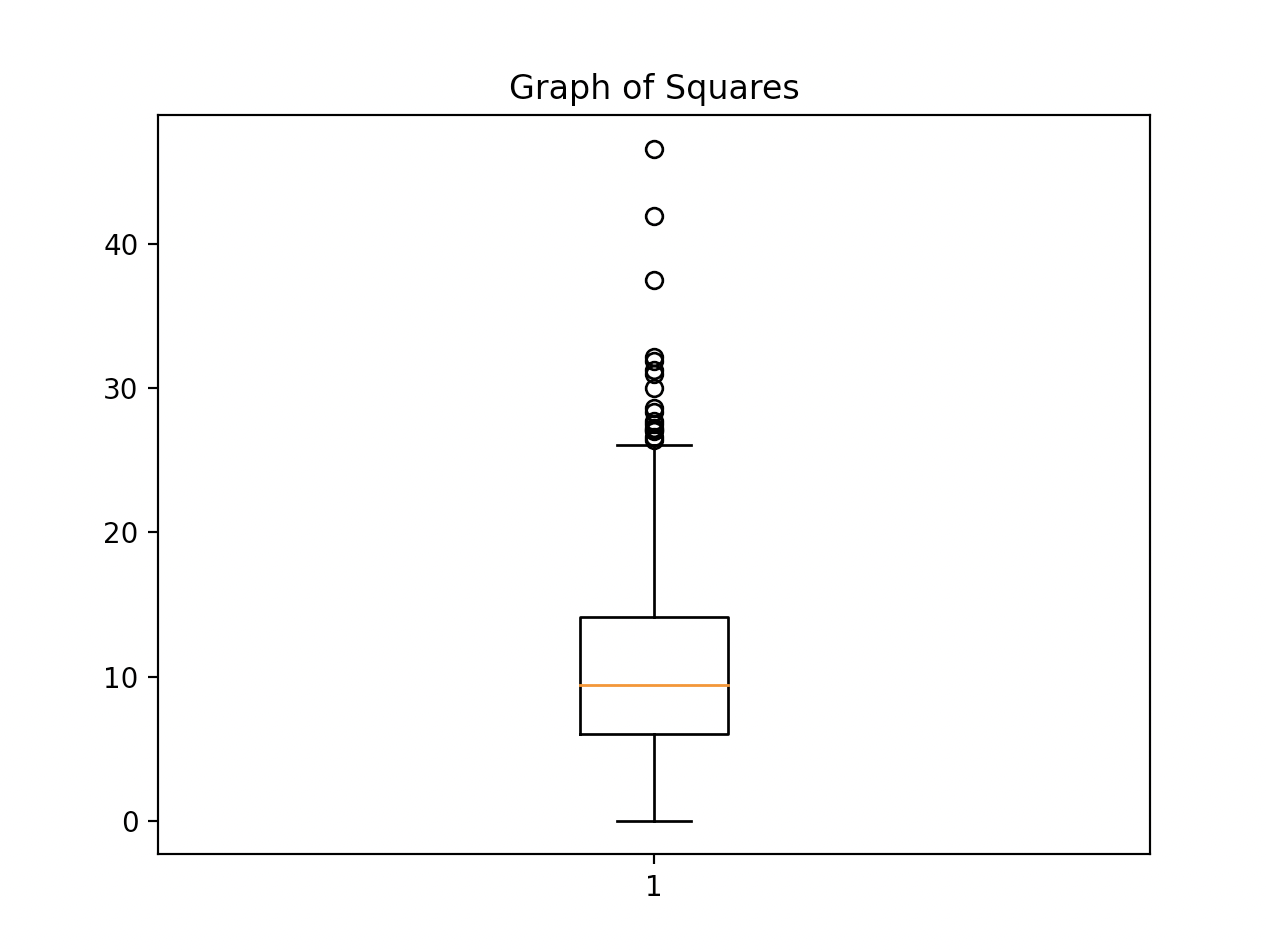
\includegraphics[scale=.33]{box_plot}
    \]  
    \item [(d)] Finally, we can compute the precise numerical statistics 
        that our boxplot helps us visualize. We will compute the first quartile, 
        median, and thhird quartile. Using the python script 
\begin{lstlisting}[language=python]
    median = round(np.percentile(xSquares, 50), 3)
    firstQ = round(np.percentile(xSquares, 25), 3)
    thirdQ = round(np.percentile(xSquares, 75), 3)
    print(f"{'First Quartile' :<20}{'Median' :<20}{'Third Quartile' :<20}")
    print(f"{firstQ :<20}{median :<20}{thirdQ :<20}")
\end{lstlisting}
    we can get an output giving us our numerical statistics:
\begin{lstlisting}[language=python]
    >>> First Quartile    Median           Third Quartile      
    >>> 6.039             9.426            14.113 
\end{lstlisting}
\end{enumerate}
\noindent\makebox[\linewidth]{\rule{18cm}{0.4pt}}



\section*{Problem 3}
Again, as a prerequisite to the remainder of this problem, we head our python 
file with the following statements
\begin{lstlisting}[language=python]
    import numpy as np
    import matplotlib.pyplot
    from matplotlib.pyplot import show
\end{lstlisting}
Now we may begin our work.
\begin{enumerate}
    \item [(a)] We may begin by loading our data set using $\texttt{np.loadtxt}$:
\begin{lstlisting}[language=python]
    D = np.loadtxt('python_files/datasets/data.csv', delimiter = ',', skiprows=1, usecols=tuple(range(2, 13)))
\end{lstlisting}
    Unpacking this function call, we see our first parameter is a path to the CSV file. The 
    delimiter paramter lets NumPy know what character separates our data values. The skiprows 
    parameter tells NumPy to not import the data from the first row, as this is the title of each column 
    and is not a numerical value. Finally, the usecols parameter uses the standard python 
    $\texttt{tuple()}$ and $\texttt{range()}$ functions to tell NumPy to use the data from the 
    columns 2 to 12. \\ \\
    Now, we may print the shape of our array, $\texttt{D}$ by using 
\begin{lstlisting}[language=python]
    print(D.shape)
\end{lstlisting}
    which gives us the output 
\begin{lstlisting}[language=python]
    >>> (569, 11)
\end{lstlisting}
    telling us that we have 11 attributes for each data point and 569 data points in total. 
    \item [(b)] It will be helpful to visualize this data set. In particular, we are 
        concerned with the Mean Radius and Mean Texture attributes. In our array, these are
        the columns indexed 1 and 2 respectively. Using $\texttt{matplotlib.pyplot.scatter()}$, we 
        can graph these two columns on a scatterplot. We use the python code 
\begin{lstlisting}[language=python]
    matplotlib.pyplot.scatter(D[:,1], D[:,2])
    matplotlib.pyplot.xlabel("Mean Radius")
    matplotlib.pyplot.ylabel("Mean Texture")
    matplotlib.pyplot.xlim((0, max(D[:,1] + 5)))
    matplotlib.pyplot.ylim((0, max(D[:,1] + 5)))
    show()
\end{lstlisting}
    Calling $\texttt{D[:,1]}$ as the first parameter uses the second column of $D$ as our x-axis. Likewise, 
    calling $\texttt{D[:,2]}$ as the second parameter uses the third column of $D$ as the y-axis. Then we label 
    our axes and set the scale of the axes for a more helpful visualization. And finally 
    we use $\texttt{show()}$ to see the figure 
    \[
        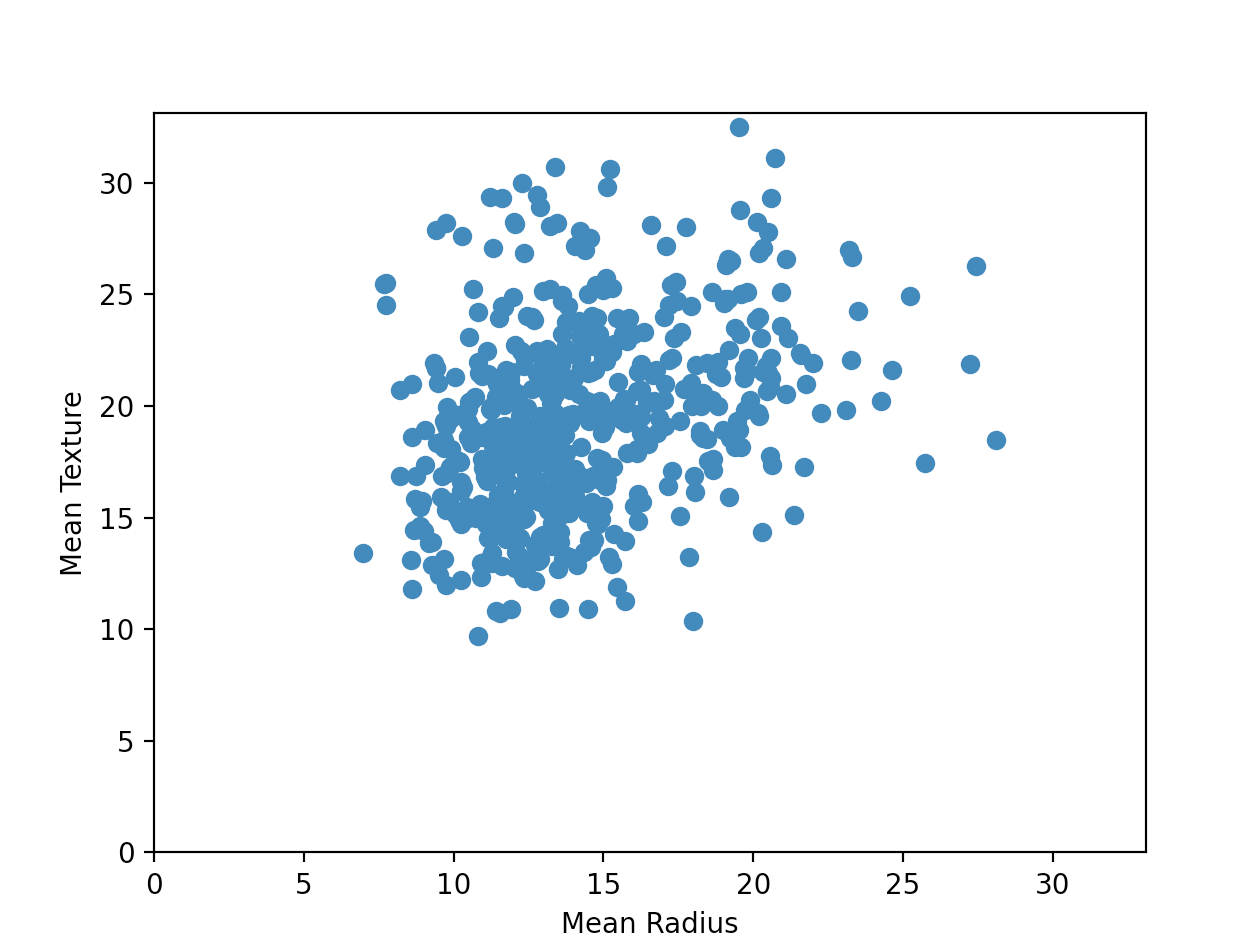
\includegraphics[scale=.33]{scatter_1.png}
    \]  
    \item[(c)] While the above scatterplot is useful, it would be more helpful 
    to be able to visualize the benign vs. malignant datapoints in seperate colors, 
    so we could attempt to make inferences about which attribute may have more of an 
    effect on predicting the severity. To do this, we must use boolean indexing to create 
    seperate Numpy arrays for the benign and malignant data sets. Our python script: 
\begin{lstlisting}[language=python]
    meanRadBenign = D[D[:,0] == 0, 1]
    meanRadMalignant = D[D[:,0] == 1, 1]
    meanTextBenign = D[D[:,0] == 0, 2]
    meanTextMalignant = D[D[:,0] == 1, 2]
    benign = matplotlib.pyplot.scatter(meanRadBenign, meanTextBenign, c=['blue'])
    malignant = matplotlib.pyplot.scatter(meanRadMalignant, meanTextMalignant, c=['red'])
    matplotlib.pyplot.xlabel("Mean Radius")
    matplotlib.pyplot.ylabel("Mean Texture")
    matplotlib.pyplot.xlim((min(D[:,1]) - 5, max(D[:,1] + 5)))
    matplotlib.pyplot.ylim((min(D[:,1]) - 5, max(D[:,1] + 5)))
    matplotlib.pyplot.legend([benign, malignant], ["Benign", "Malignant"])
    show()
\end{lstlisting}
    The first for lines initilize NumPy arrays for our four datasets, whcih are sorted by 
    their condition (benign or malignant). Next, we declare two scatter plot instances 
    whichh follow the same index as in part ${\bf b}$, using the radius attribute for the
    x-axis and the y-axis for the texture attribute. Additionally, we added the c parameter, 
    to declare the color of our data points. In the benign scatter plot, our datapoints are blue, 
    while in the malignant plot, our data points are red. Then we label the axes and set the scale, 
    and finally we view our figure 
    \[
        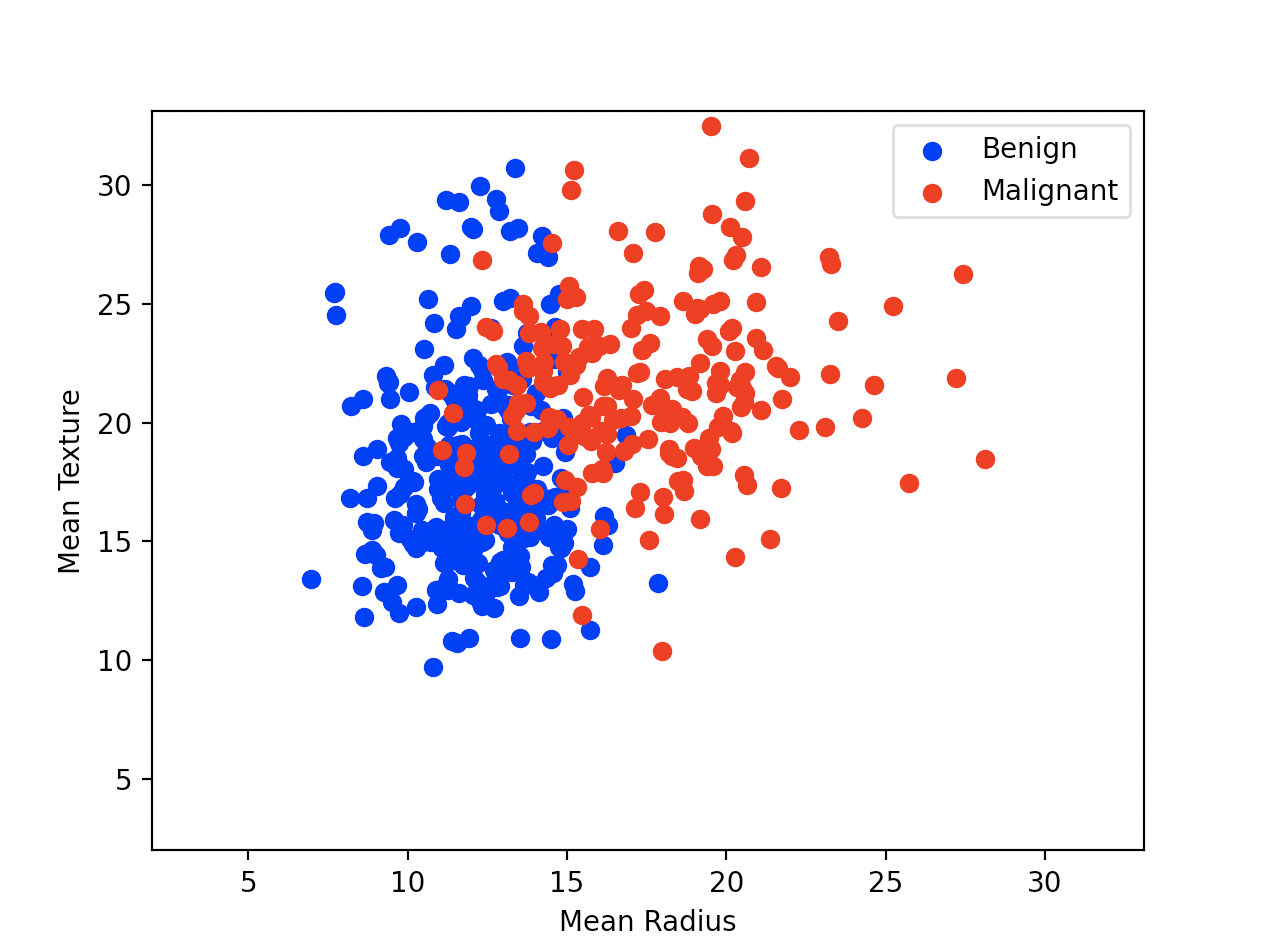
\includegraphics[scale = .33]{scatter_2.png}
    \]  
    \item [(d)] Based on the scatterplots generated in parts ${\bf b}$ and ${\bf c}$, 
        it seems as though it would be possible to make predictions about a patients conditions 
        based on radius and texture measurements. \\ \\
        In most cases, with a mean radius less than 15 and mean texture less than 20, 
        I feel it would be a safe guess to give a benign diagnosis. On the other hand, in instances 
        where the mean radius is greater than 15 and the mean texture is greater than 20, I believe 
        it would be safe to give a malignant diagnosis. \\ \\
        In the edge cases where only one of these conditions is satisfied, but not the other, 
        more analysis of additional attributes could be helpful. \\ \\
        If I had to pick one attribute to more accurately predict diagnosis, 
        I would likely select radius, as there seems to me a more dichotomous division across the 
        x-axis than across the y-axis.
\end{enumerate}
\noindent\makebox[\linewidth]{\rule{18cm}{0.4pt}}

\section*{Problem 4}
\begin{enumerate}
    \item [(a)] Let us take a look at the python script and then unpack it step by step:
\begin{lstlisting}[language=python]
    import numpy as np

    D = np.loadtxt('python_files/datasets/data.csv', delimiter = ',', skiprows=1, usecols=tuple(range(2, 13)))
    desc = D[:,[1,2,3,4,5,6,7,8,9,10]]
    meanDesc = np.mean(desc, axis=0)
    
    for size in range(0, 6):
        N = 10 * (2 ** size) #sample size
        sample = np.empty((0,10))
        normSamp = []
        for _ in range(10001):
            sample = desc[np.random.choice(desc.shape[0], size=N, replace=True), :]
            meanSamp = np.mean(sample, axis=0)
            dist = abs(meanSamp - meanDesc)
            normSamp.append(np.linalg.norm(dist))
        normSamp = np.array(normSamp)
        print(f"({N}, {np.mean(normSamp)})")
\end{lstlisting}
    As in question ${\bf 3}$, we begin by loading our dataset. Then, we create a second array, 
    $\texttt{desc}$, which contains only the descriptive attributes and compute the mean across 
    the x-axis, which produces 1D array of length 10, containing the mean value of each descriptive 
    attribute. These values will be used later in our loops. \\ \\
    Our outer loop while iterate over our values of $\texttt{p}$. For each of these values it will 
    compute an $\texttt{N}$ sample size and initilize an empty sample 1D array of length 10. Additionally, 
    we will initialize an empty list to hold norm values of each sample. \\ \\
    Then, our inner loop will iterate 10,000 times. With each iteration, we will create an NumPy array, 
    $\texttt{sample}$, which holds our $\texttt{N}$ randomly selected rows. We will take the mean of this 
    sample and then take the norm value of the difference of the sample mean and the mean of the total dataset. 
    Note the use of the vectorized subtraction in line 14 to easily calculate the distance. \\ \\
    Finally, after our inner loop completes, we have a list, $\texttt{normSamp}$ of length 10,000, which we
    quickly convert to a 1D NumPy array so that we can take the mean. Finally, we print the results of each 
    iteration in a tuple of the form 
    \[
        \text{ (N, mean of norm values)}
    \]  
    After running this script, we get an output of 
\begin{lstlisting}[language=python]
    >>> (10, 88.96267114841969)
    >>> (20, 62.6722197836738)
    >>> (40, 44.631940662004176)
    >>> (80, 31.083888414534048)
    >>> (160, 22.16534548078403)
    >>> (320, 15.679423991364414)
\end{lstlisting}
    \item [(b)] As the size of our sample grows, the mean vector decreases. This suggests that as we 
        take larger and larger sample sizes, the samples we select become more and more accurate relative 
        relative to the entire dataset. \\ \\ 
        This makes sense, because as we select larger and larger samples of data, the chances that we can 
        outweigh the effects of outliers in our samples become much higher. As a result, with a larger sample 
        size, the data is closer to the whole data set. 
    \item [(c)] In addition, we can actually qualitatively analyze the relationship between 
        differences in our sample means. Using the following equation 
        \[
            \text{norm for sample N } = (\frac{N}{10})^p * (\text{norm for N = 10})
        \]  
        We can try to solve for $p$ by plugging in values 
        \begin{align}
            89 &= (\frac{10}{10})^p * 89  &\implies p = -.49\\ 
            63 &= (\frac{20}{10})^p * 89 &\implies p = -.51\\ 
            44 &= (\frac{40}{10})^p * 89 &\implies p = -.51\\ 
            31 &= (\frac{80}{10})^p * 89 &\implies p = -.50\\ 
            22 &= (\frac{160}{10})^p * 89 &\implies p = -.50\\ 
            16 &= (\frac{320}{10})^p * 89 &\implies p = -.50
        \end{align}
        We can see that if multiply $N$ by 4, (looking at lines (1) and (3)) our norm 
        value is divided by 2. \\ \\
        From this data we can see that our value for $p$ is $-\frac{1}{2}$. 
\end{enumerate}




\end{document}